% Options for packages loaded elsewhere
\PassOptionsToPackage{unicode}{hyperref}
\PassOptionsToPackage{hyphens}{url}
\PassOptionsToPackage{dvipsnames,svgnames,x11names}{xcolor}
%
\documentclass[
  letterpaper,
  DIV=11,
  numbers=noendperiod]{scrartcl}

\usepackage{amsmath,amssymb}
\usepackage{iftex}
\ifPDFTeX
  \usepackage[T1]{fontenc}
  \usepackage[utf8]{inputenc}
  \usepackage{textcomp} % provide euro and other symbols
\else % if luatex or xetex
  \usepackage{unicode-math}
  \defaultfontfeatures{Scale=MatchLowercase}
  \defaultfontfeatures[\rmfamily]{Ligatures=TeX,Scale=1}
\fi
\usepackage{lmodern}
\ifPDFTeX\else  
    % xetex/luatex font selection
\fi
% Use upquote if available, for straight quotes in verbatim environments
\IfFileExists{upquote.sty}{\usepackage{upquote}}{}
\IfFileExists{microtype.sty}{% use microtype if available
  \usepackage[]{microtype}
  \UseMicrotypeSet[protrusion]{basicmath} % disable protrusion for tt fonts
}{}
\makeatletter
\@ifundefined{KOMAClassName}{% if non-KOMA class
  \IfFileExists{parskip.sty}{%
    \usepackage{parskip}
  }{% else
    \setlength{\parindent}{0pt}
    \setlength{\parskip}{6pt plus 2pt minus 1pt}}
}{% if KOMA class
  \KOMAoptions{parskip=half}}
\makeatother
\usepackage{xcolor}
\setlength{\emergencystretch}{3em} % prevent overfull lines
\setcounter{secnumdepth}{-\maxdimen} % remove section numbering
% Make \paragraph and \subparagraph free-standing
\makeatletter
\ifx\paragraph\undefined\else
  \let\oldparagraph\paragraph
  \renewcommand{\paragraph}{
    \@ifstar
      \xxxParagraphStar
      \xxxParagraphNoStar
  }
  \newcommand{\xxxParagraphStar}[1]{\oldparagraph*{#1}\mbox{}}
  \newcommand{\xxxParagraphNoStar}[1]{\oldparagraph{#1}\mbox{}}
\fi
\ifx\subparagraph\undefined\else
  \let\oldsubparagraph\subparagraph
  \renewcommand{\subparagraph}{
    \@ifstar
      \xxxSubParagraphStar
      \xxxSubParagraphNoStar
  }
  \newcommand{\xxxSubParagraphStar}[1]{\oldsubparagraph*{#1}\mbox{}}
  \newcommand{\xxxSubParagraphNoStar}[1]{\oldsubparagraph{#1}\mbox{}}
\fi
\makeatother

\usepackage{color}
\usepackage{fancyvrb}
\newcommand{\VerbBar}{|}
\newcommand{\VERB}{\Verb[commandchars=\\\{\}]}
\DefineVerbatimEnvironment{Highlighting}{Verbatim}{commandchars=\\\{\}}
% Add ',fontsize=\small' for more characters per line
\usepackage{framed}
\definecolor{shadecolor}{RGB}{241,243,245}
\newenvironment{Shaded}{\begin{snugshade}}{\end{snugshade}}
\newcommand{\AlertTok}[1]{\textcolor[rgb]{0.68,0.00,0.00}{#1}}
\newcommand{\AnnotationTok}[1]{\textcolor[rgb]{0.37,0.37,0.37}{#1}}
\newcommand{\AttributeTok}[1]{\textcolor[rgb]{0.40,0.45,0.13}{#1}}
\newcommand{\BaseNTok}[1]{\textcolor[rgb]{0.68,0.00,0.00}{#1}}
\newcommand{\BuiltInTok}[1]{\textcolor[rgb]{0.00,0.23,0.31}{#1}}
\newcommand{\CharTok}[1]{\textcolor[rgb]{0.13,0.47,0.30}{#1}}
\newcommand{\CommentTok}[1]{\textcolor[rgb]{0.37,0.37,0.37}{#1}}
\newcommand{\CommentVarTok}[1]{\textcolor[rgb]{0.37,0.37,0.37}{\textit{#1}}}
\newcommand{\ConstantTok}[1]{\textcolor[rgb]{0.56,0.35,0.01}{#1}}
\newcommand{\ControlFlowTok}[1]{\textcolor[rgb]{0.00,0.23,0.31}{\textbf{#1}}}
\newcommand{\DataTypeTok}[1]{\textcolor[rgb]{0.68,0.00,0.00}{#1}}
\newcommand{\DecValTok}[1]{\textcolor[rgb]{0.68,0.00,0.00}{#1}}
\newcommand{\DocumentationTok}[1]{\textcolor[rgb]{0.37,0.37,0.37}{\textit{#1}}}
\newcommand{\ErrorTok}[1]{\textcolor[rgb]{0.68,0.00,0.00}{#1}}
\newcommand{\ExtensionTok}[1]{\textcolor[rgb]{0.00,0.23,0.31}{#1}}
\newcommand{\FloatTok}[1]{\textcolor[rgb]{0.68,0.00,0.00}{#1}}
\newcommand{\FunctionTok}[1]{\textcolor[rgb]{0.28,0.35,0.67}{#1}}
\newcommand{\ImportTok}[1]{\textcolor[rgb]{0.00,0.46,0.62}{#1}}
\newcommand{\InformationTok}[1]{\textcolor[rgb]{0.37,0.37,0.37}{#1}}
\newcommand{\KeywordTok}[1]{\textcolor[rgb]{0.00,0.23,0.31}{\textbf{#1}}}
\newcommand{\NormalTok}[1]{\textcolor[rgb]{0.00,0.23,0.31}{#1}}
\newcommand{\OperatorTok}[1]{\textcolor[rgb]{0.37,0.37,0.37}{#1}}
\newcommand{\OtherTok}[1]{\textcolor[rgb]{0.00,0.23,0.31}{#1}}
\newcommand{\PreprocessorTok}[1]{\textcolor[rgb]{0.68,0.00,0.00}{#1}}
\newcommand{\RegionMarkerTok}[1]{\textcolor[rgb]{0.00,0.23,0.31}{#1}}
\newcommand{\SpecialCharTok}[1]{\textcolor[rgb]{0.37,0.37,0.37}{#1}}
\newcommand{\SpecialStringTok}[1]{\textcolor[rgb]{0.13,0.47,0.30}{#1}}
\newcommand{\StringTok}[1]{\textcolor[rgb]{0.13,0.47,0.30}{#1}}
\newcommand{\VariableTok}[1]{\textcolor[rgb]{0.07,0.07,0.07}{#1}}
\newcommand{\VerbatimStringTok}[1]{\textcolor[rgb]{0.13,0.47,0.30}{#1}}
\newcommand{\WarningTok}[1]{\textcolor[rgb]{0.37,0.37,0.37}{\textit{#1}}}

\providecommand{\tightlist}{%
  \setlength{\itemsep}{0pt}\setlength{\parskip}{0pt}}\usepackage{longtable,booktabs,array}
\usepackage{calc} % for calculating minipage widths
% Correct order of tables after \paragraph or \subparagraph
\usepackage{etoolbox}
\makeatletter
\patchcmd\longtable{\par}{\if@noskipsec\mbox{}\fi\par}{}{}
\makeatother
% Allow footnotes in longtable head/foot
\IfFileExists{footnotehyper.sty}{\usepackage{footnotehyper}}{\usepackage{footnote}}
\makesavenoteenv{longtable}
\usepackage{graphicx}
\makeatletter
\def\maxwidth{\ifdim\Gin@nat@width>\linewidth\linewidth\else\Gin@nat@width\fi}
\def\maxheight{\ifdim\Gin@nat@height>\textheight\textheight\else\Gin@nat@height\fi}
\makeatother
% Scale images if necessary, so that they will not overflow the page
% margins by default, and it is still possible to overwrite the defaults
% using explicit options in \includegraphics[width, height, ...]{}
\setkeys{Gin}{width=\maxwidth,height=\maxheight,keepaspectratio}
% Set default figure placement to htbp
\makeatletter
\def\fps@figure{htbp}
\makeatother
% definitions for citeproc citations
\NewDocumentCommand\citeproctext{}{}
\NewDocumentCommand\citeproc{mm}{%
  \begingroup\def\citeproctext{#2}\cite{#1}\endgroup}
\makeatletter
 % allow citations to break across lines
 \let\@cite@ofmt\@firstofone
 % avoid brackets around text for \cite:
 \def\@biblabel#1{}
 \def\@cite#1#2{{#1\if@tempswa , #2\fi}}
\makeatother
\newlength{\cslhangindent}
\setlength{\cslhangindent}{1.5em}
\newlength{\csllabelwidth}
\setlength{\csllabelwidth}{3em}
\newenvironment{CSLReferences}[2] % #1 hanging-indent, #2 entry-spacing
 {\begin{list}{}{%
  \setlength{\itemindent}{0pt}
  \setlength{\leftmargin}{0pt}
  \setlength{\parsep}{0pt}
  % turn on hanging indent if param 1 is 1
  \ifodd #1
   \setlength{\leftmargin}{\cslhangindent}
   \setlength{\itemindent}{-1\cslhangindent}
  \fi
  % set entry spacing
  \setlength{\itemsep}{#2\baselineskip}}}
 {\end{list}}
\usepackage{calc}
\newcommand{\CSLBlock}[1]{\hfill\break\parbox[t]{\linewidth}{\strut\ignorespaces#1\strut}}
\newcommand{\CSLLeftMargin}[1]{\parbox[t]{\csllabelwidth}{\strut#1\strut}}
\newcommand{\CSLRightInline}[1]{\parbox[t]{\linewidth - \csllabelwidth}{\strut#1\strut}}
\newcommand{\CSLIndent}[1]{\hspace{\cslhangindent}#1}

\KOMAoption{captions}{tableheading}
\makeatletter
\@ifpackageloaded{caption}{}{\usepackage{caption}}
\AtBeginDocument{%
\ifdefined\contentsname
  \renewcommand*\contentsname{Table of contents}
\else
  \newcommand\contentsname{Table of contents}
\fi
\ifdefined\listfigurename
  \renewcommand*\listfigurename{List of Figures}
\else
  \newcommand\listfigurename{List of Figures}
\fi
\ifdefined\listtablename
  \renewcommand*\listtablename{List of Tables}
\else
  \newcommand\listtablename{List of Tables}
\fi
\ifdefined\figurename
  \renewcommand*\figurename{Figure}
\else
  \newcommand\figurename{Figure}
\fi
\ifdefined\tablename
  \renewcommand*\tablename{Table}
\else
  \newcommand\tablename{Table}
\fi
}
\@ifpackageloaded{float}{}{\usepackage{float}}
\floatstyle{ruled}
\@ifundefined{c@chapter}{\newfloat{codelisting}{h}{lop}}{\newfloat{codelisting}{h}{lop}[chapter]}
\floatname{codelisting}{Listing}
\newcommand*\listoflistings{\listof{codelisting}{List of Listings}}
\makeatother
\makeatletter
\makeatother
\makeatletter
\@ifpackageloaded{caption}{}{\usepackage{caption}}
\@ifpackageloaded{subcaption}{}{\usepackage{subcaption}}
\makeatother

\ifLuaTeX
  \usepackage{selnolig}  % disable illegal ligatures
\fi
\usepackage{bookmark}

\IfFileExists{xurl.sty}{\usepackage{xurl}}{} % add URL line breaks if available
\urlstyle{same} % disable monospaced font for URLs
\hypersetup{
  pdftitle={Assignment 2: Regression models, predicting from data},
  colorlinks=true,
  linkcolor={blue},
  filecolor={Maroon},
  citecolor={Blue},
  urlcolor={Blue},
  pdfcreator={LaTeX via pandoc}}


\title{Assignment 2: Regression models, predicting from data}
\author{}
\date{}

\begin{document}
\maketitle


\subsection{Introduksjon / Bakgrunn}\label{introduksjon-bakgrunn}

Denne oppgaven er delt inn tre separate deler som tar for seg konsepter
innenfor analyse av data og regresjon. I del 1 kalkulerer vi laktat
terskler, og ser nærmere på reliabiliteten mellom to ulike
terskelnivåer. Del 2 bruker vi molekylær data til å predikere størrelsen
på DNA-fragment ved hjelp av en veileder. I del 3 skal vi se nærmere på
om det finnes en lineær sammenheng mellom to valgte variabler fra
datasettet \texttt{hypertrophy}i datapakken \texttt{exscidata}.

\subsection{Del 1: Laktat terskler}\label{del-1-laktat-terskler}

\subsubsection{Introduksjon}\label{introduksjon}

Laktat terskel er en variabel som er godt brukt for å forutsi prestasjon
innenfor utholdenhets idretter, til å styre intensiteten av
treningsøkter og evaluere trenings effekt (Machado et al., 2012). Det
finnes ulike metoder for å finne testpersonens laktat terskel. Machado
et al. (2012) forteller oss at den ``maximal-deviation method'' (Dmax)
anbefalt av Cheng et al.~1992, bidrar med å kunne evaluere de ulike
mekanismene som virker bestemmende for prestasjon innenfor
langdistanseløping og sykling (Machado et al., 2012). Videre hadde denne
metoden en bedre korrelasjon med prestasjon og laktat terskel
sammenliknet med andre metoder. I våres reliabilitets tester ble det
ikke utført laktat målinger, på bakgrunn av dette benytter vi oss av
data settet til ``cyclingstudy''. De representative tersklene som blir
undersøkt er 2 mmol L-1 og 4 mmol L-1.

\subsubsection{Metode}\label{metode}

Som en kan se i den plotta grafen under, er de forskjellige grafene ikke
så forskjellige rundt 2mmol og 4mmol L\textasciitilde-1. På den andre
siden ser vi at den lineære modellen er feil ved 300w, den
sekundærplynomiske modellen er feil ved 275w. Den tredje- og
fjerdeplynomiske modellen derimot, varierer ikke mye fra hverandre.

\begin{Shaded}
\begin{Highlighting}[]
\DocumentationTok{\#\#\# laste ned nødvendige packages}
\FunctionTok{library}\NormalTok{(tidyr)}
\FunctionTok{library}\NormalTok{(tidyverse)}
\FunctionTok{library}\NormalTok{(ggplot2)}
\FunctionTok{library}\NormalTok{(exscidata)}


\DocumentationTok{\#\#\#laste inn data}
\FunctionTok{data}\NormalTok{(}\StringTok{"cyclingstudy"}\NormalTok{)}


\DocumentationTok{\#\#\# Estimering av laktatterskelen og treningsintensiteten ved 4mmol L{-}1 }

\NormalTok{cyclingstudy }\SpecialCharTok{\%\textgreater{}\%}
  \CommentTok{\# utvalg av nødvendige kolonner i analysen.}
  \FunctionTok{select}\NormalTok{(subject, group, timepoint, lac}\FloatTok{.225}\SpecialCharTok{:}\NormalTok{lac}\FloatTok{.375}\NormalTok{) }\SpecialCharTok{\%\textgreater{}\%}
  \CommentTok{\# Kun ein deltaker og ett tidspunkt.}
  \FunctionTok{filter}\NormalTok{(timepoint }\SpecialCharTok{==} \StringTok{"pre"}\NormalTok{, subject }\SpecialCharTok{==} \DecValTok{10}\NormalTok{) }\SpecialCharTok{\%\textgreater{}\%}
  \CommentTok{\# lang format ved å bruke laktatkolonnene.}
  \FunctionTok{pivot\_longer}\NormalTok{(}\AttributeTok{names\_to =} \StringTok{"watt"}\NormalTok{,}
               \AttributeTok{values\_to =} \StringTok{"lactate"}\NormalTok{,}
               \AttributeTok{names\_prefix =} \StringTok{"lac."}\NormalTok{,}
               \AttributeTok{names\_transform =} \FunctionTok{list}\NormalTok{(}\AttributeTok{watt =}\NormalTok{ as.numeric),}
               \AttributeTok{cols =}\NormalTok{ lac}\FloatTok{.225}\SpecialCharTok{:}\NormalTok{lac}\FloatTok{.375}\NormalTok{) }\SpecialCharTok{\%\textgreater{}\%}
  \CommentTok{\# Plotte data, group = subject nødvendig for å sammenkoble punktene.}
  \FunctionTok{ggplot}\NormalTok{(}\FunctionTok{aes}\NormalTok{(watt, lactate, }\AttributeTok{group =}\NormalTok{ subject)) }\SpecialCharTok{+}
  \FunctionTok{geom\_line}\NormalTok{(}\AttributeTok{lty =} \DecValTok{2}\NormalTok{) }\SpecialCharTok{+}
  \FunctionTok{geom\_point}\NormalTok{(}\AttributeTok{shape =} \DecValTok{21}\NormalTok{, }\AttributeTok{fill =} \StringTok{"lightblue"}\NormalTok{, }\AttributeTok{size =} \FloatTok{2.5}\NormalTok{) }\SpecialCharTok{+}
  \CommentTok{\# Linjer på spesifikke punktene for 2mmol og 4mmol, samt skjeringspunktet mellom linjene.}
  \FunctionTok{geom\_hline}\NormalTok{(}\AttributeTok{yintercept =} \DecValTok{4}\NormalTok{, }\AttributeTok{color =} \StringTok{"red"}\NormalTok{) }\SpecialCharTok{+}
  \FunctionTok{geom\_hline}\NormalTok{(}\AttributeTok{yintercept =} \DecValTok{2}\NormalTok{, }\AttributeTok{color =} \StringTok{"gold"}\NormalTok{) }\SpecialCharTok{+}
  \FunctionTok{geom\_vline}\NormalTok{(}\AttributeTok{xintercept =} \FloatTok{341.5}\NormalTok{, }\AttributeTok{color =} \StringTok{"blue"}\NormalTok{) }\SpecialCharTok{+}
  \FunctionTok{geom\_vline}\NormalTok{(}\AttributeTok{xintercept =} \DecValTok{308}\NormalTok{, }\AttributeTok{color =} \StringTok{"green"}\NormalTok{) }\SpecialCharTok{+}
  \CommentTok{\# legge til en strak linje fra den lineære modelen.}
  \FunctionTok{geom\_smooth}\NormalTok{(}\AttributeTok{method =} \StringTok{"lm"}\NormalTok{, }\AttributeTok{se =} \ConstantTok{FALSE}\NormalTok{, }\AttributeTok{formula =}\NormalTok{ y }\SpecialCharTok{\textasciitilde{}}\NormalTok{ x, }\AttributeTok{color =} \StringTok{"\#e41a1c"}\NormalTok{) }\SpecialCharTok{+}
  
  \CommentTok{\# poly(x, 2) Legger til en andregradsplynomisk modell.}
  \FunctionTok{geom\_smooth}\NormalTok{(}\AttributeTok{method =} \StringTok{"lm"}\NormalTok{, }\AttributeTok{se =} \ConstantTok{FALSE}\NormalTok{, }\AttributeTok{formula =}\NormalTok{ y }\SpecialCharTok{\textasciitilde{}} \FunctionTok{poly}\NormalTok{(x, }\DecValTok{2}\NormalTok{), }\AttributeTok{color =} \StringTok{"\#377eb8"}\NormalTok{) }\SpecialCharTok{+}
  \CommentTok{\# poly(x, 3) Legger til en tredjegradsplynomisk modell.}
  \FunctionTok{geom\_smooth}\NormalTok{(}\AttributeTok{method =} \StringTok{"lm"}\NormalTok{, }\AttributeTok{se =} \ConstantTok{FALSE}\NormalTok{, }\AttributeTok{formula =}\NormalTok{ y }\SpecialCharTok{\textasciitilde{}} \FunctionTok{poly}\NormalTok{(x, }\DecValTok{3}\NormalTok{), }\AttributeTok{color =} \StringTok{"\#4daf4a"}\NormalTok{) }\SpecialCharTok{+}
  \CommentTok{\# poly(x, 4) Legger til en fjerdegradsplynomisk modell.}
  \FunctionTok{geom\_smooth}\NormalTok{(}\AttributeTok{method =} \StringTok{"lm"}\NormalTok{, }\AttributeTok{se =} \ConstantTok{FALSE}\NormalTok{, }\AttributeTok{formula =}\NormalTok{ y }\SpecialCharTok{\textasciitilde{}} \FunctionTok{poly}\NormalTok{(x, }\DecValTok{4}\NormalTok{), }\AttributeTok{color =} \StringTok{"\#ff7f00"}\NormalTok{)}
\end{Highlighting}
\end{Shaded}

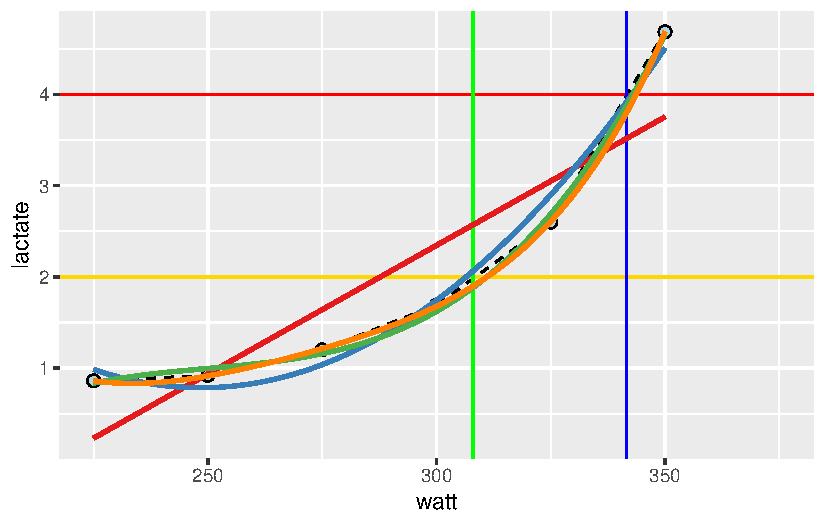
\includegraphics{02-regression-models_files/figure-pdf/unnamed-chunk-1-1.pdf}

\begin{Shaded}
\begin{Highlighting}[]
\DocumentationTok{\#\#\# vurdering av tilpasningen til de forskjellige lineære modellene på sammenhengen mellom treningsintensitet og laktatakkumulering.}

\NormalTok{lactate }\OtherTok{\textless{}{-}}\NormalTok{ cyclingstudy }\SpecialCharTok{\%\textgreater{}\%}
  \CommentTok{\# utvalg av nødvendige kolonner i analysen.}
  \FunctionTok{select}\NormalTok{(subject, group, timepoint, lac}\FloatTok{.225}\SpecialCharTok{:}\NormalTok{lac}\FloatTok{.375}\NormalTok{) }\SpecialCharTok{\%\textgreater{}\%}
  \CommentTok{\# Kun ein deltaker og ett tidspunkt.}
  \FunctionTok{filter}\NormalTok{(timepoint }\SpecialCharTok{==} \StringTok{"pre"}\NormalTok{, subject }\SpecialCharTok{==} \DecValTok{10}\NormalTok{) }\SpecialCharTok{\%\textgreater{}\%}
  \CommentTok{\# lang format ved å bruke laktatkolonnene.}
  \FunctionTok{pivot\_longer}\NormalTok{(}\AttributeTok{names\_to =} \StringTok{"watt"}\NormalTok{,}
               \AttributeTok{values\_to =} \StringTok{"lactate"}\NormalTok{,}
               \AttributeTok{names\_prefix =} \StringTok{"lac."}\NormalTok{,}
               \AttributeTok{names\_transform =} \FunctionTok{list}\NormalTok{(}\AttributeTok{watt =}\NormalTok{ as.numeric),}
               \AttributeTok{cols =}\NormalTok{ lac}\FloatTok{.225}\SpecialCharTok{:}\NormalTok{lac}\FloatTok{.375}\NormalTok{) }\SpecialCharTok{\%\textgreater{}\%}
  \CommentTok{\# Fjerne dei ugyldige veriene NA for å hindre feilmeldinger.}
  \FunctionTok{filter}\NormalTok{(}\SpecialCharTok{!}\FunctionTok{is.na}\NormalTok{(lactate))}

\CommentTok{\# Legger til en strak linje fra modelen.}
\NormalTok{m1 }\OtherTok{\textless{}{-}} \FunctionTok{lm}\NormalTok{(lactate }\SpecialCharTok{\textasciitilde{}}\NormalTok{ watt, }\AttributeTok{data =}\NormalTok{ lactate)}

\CommentTok{\# Legger til en andregradsplynomisk modell.}
\NormalTok{m2 }\OtherTok{\textless{}{-}} \FunctionTok{lm}\NormalTok{(lactate }\SpecialCharTok{\textasciitilde{}} \FunctionTok{poly}\NormalTok{(watt, }\DecValTok{2}\NormalTok{, }\AttributeTok{raw =} \ConstantTok{TRUE}\NormalTok{), }\AttributeTok{data =}\NormalTok{ lactate)}

\CommentTok{\# Legger til en tredjegradsplynomisk modell.}
\NormalTok{m3 }\OtherTok{\textless{}{-}} \FunctionTok{lm}\NormalTok{(lactate }\SpecialCharTok{\textasciitilde{}} \FunctionTok{poly}\NormalTok{(watt, }\DecValTok{3}\NormalTok{, }\AttributeTok{raw =} \ConstantTok{TRUE}\NormalTok{), }\AttributeTok{data =}\NormalTok{ lactate)}

\CommentTok{\# Legger til en fjerdegradsplynomisk modell.}
\NormalTok{m4 }\OtherTok{\textless{}{-}} \FunctionTok{lm}\NormalTok{(lactate }\SpecialCharTok{\textasciitilde{}} \FunctionTok{poly}\NormalTok{(watt, }\DecValTok{4}\NormalTok{, }\AttributeTok{raw =} \ConstantTok{TRUE}\NormalTok{), }\AttributeTok{data =}\NormalTok{ lactate)}

\CommentTok{\# Lagre alle restverdiene som nye variabler.}
\NormalTok{lactate}\SpecialCharTok{$}\NormalTok{resid.m1 }\OtherTok{\textless{}{-}} \FunctionTok{resid}\NormalTok{(m1)}
\NormalTok{lactate}\SpecialCharTok{$}\NormalTok{resid.m2 }\OtherTok{\textless{}{-}} \FunctionTok{resid}\NormalTok{(m2)}
\NormalTok{lactate}\SpecialCharTok{$}\NormalTok{resid.m3 }\OtherTok{\textless{}{-}} \FunctionTok{resid}\NormalTok{(m3)}
\NormalTok{lactate}\SpecialCharTok{$}\NormalTok{resid.m4 }\OtherTok{\textless{}{-}} \FunctionTok{resid}\NormalTok{(m4)}

\NormalTok{lactate }\SpecialCharTok{\%\textgreater{}\%}
  \CommentTok{\# Samle all data fra modelleme.}
  \FunctionTok{pivot\_longer}\NormalTok{(}\AttributeTok{names\_to =} \StringTok{"model"}\NormalTok{,}
               \AttributeTok{values\_to =} \StringTok{"residual"}\NormalTok{,}
               \AttributeTok{names\_prefix =} \StringTok{"resid."}\NormalTok{,}
               \AttributeTok{names\_transform =} \FunctionTok{list}\NormalTok{(}\AttributeTok{residual =}\NormalTok{ as.numeric),}
               \AttributeTok{cols =}\NormalTok{ resid.m1}\SpecialCharTok{:}\NormalTok{resid.m4) }\SpecialCharTok{\%\textgreater{}\%}
  \CommentTok{\# Plotte verdiene fra den observerte watten på x aksen og restverdiene på y aksen}
  \FunctionTok{ggplot}\NormalTok{(}\FunctionTok{aes}\NormalTok{(watt, residual, }\AttributeTok{fill =}\NormalTok{ model)) }\SpecialCharTok{+} \FunctionTok{geom\_point}\NormalTok{(}\AttributeTok{shape =} \DecValTok{21}\NormalTok{, }\AttributeTok{size =} \DecValTok{3}\NormalTok{) }\SpecialCharTok{+}
  
  \CommentTok{\# For å ha samme farger som over, bruker me scale fill manual.}
  \FunctionTok{scale\_fill\_manual}\NormalTok{(}\AttributeTok{values =} \FunctionTok{c}\NormalTok{(}\StringTok{"\#e41a1c"}\NormalTok{, }\StringTok{"\#377eb8"}\NormalTok{, }\StringTok{"\#4daf4a"}\NormalTok{, }\StringTok{"\#ff7f00"}\NormalTok{))}
\end{Highlighting}
\end{Shaded}

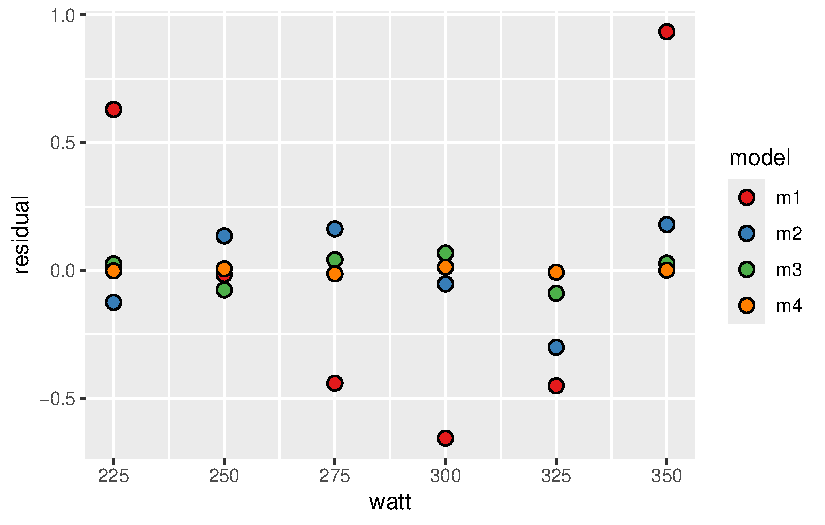
\includegraphics{02-regression-models_files/figure-pdf/unnamed-chunk-2-1.pdf}

For å finne ut hva forutsatt wattverdi som er nærmest 2 og 4 mmol L-1,
benytter vi koden under:

\begin{Shaded}
\begin{Highlighting}[]
\CommentTok{\# Ny dataramme}
\NormalTok{ndf }\OtherTok{\textless{}{-}} \FunctionTok{data.frame}\NormalTok{(}\AttributeTok{watt =} \FunctionTok{seq}\NormalTok{(}\AttributeTok{from =} \DecValTok{225}\NormalTok{, }\AttributeTok{to =} \DecValTok{350}\NormalTok{, }\AttributeTok{by =} \FloatTok{0.1}\NormalTok{))}

\NormalTok{ndf}\SpecialCharTok{$}\NormalTok{predictions }\OtherTok{\textless{}{-}} \FunctionTok{predict}\NormalTok{(m3, }\AttributeTok{newdata =}\NormalTok{ ndf)}


\CommentTok{\# for å finne ut kva forutsatt Wattverdi som er nermest 2 og 4 mmol L{-}1}
\NormalTok{lactate\_threshold }\OtherTok{\textless{}{-}}\NormalTok{ ndf }\SpecialCharTok{\%\textgreater{}\%}
  \FunctionTok{filter}\NormalTok{(}\FunctionTok{abs}\NormalTok{(predictions }\SpecialCharTok{{-}} \DecValTok{4}\NormalTok{) }\SpecialCharTok{==} \FunctionTok{min}\NormalTok{(}\FunctionTok{abs}\NormalTok{(predictions }\SpecialCharTok{{-}} \DecValTok{4}\NormalTok{)))}

\FunctionTok{summary}\NormalTok{(lactate\_threshold)}
\end{Highlighting}
\end{Shaded}

\begin{verbatim}
      watt      predictions
 Min.   :343   Min.   :4   
 1st Qu.:343   1st Qu.:4   
 Median :343   Median :4   
 Mean   :343   Mean   :4   
 3rd Qu.:343   3rd Qu.:4   
 Max.   :343   Max.   :4   
\end{verbatim}

Her finner vi ut av at på 2 mmol får vi en wattverdi på 311 W, mens på 4
mmol får vi en wattverdi på 343 W. Verdien for 2 mmol ligg på samme
dataframe som kjem fram på 4 mmol L-1.

\subsection{Del 2: Forutsi størrelser på DNA fragmenter eller stiningene
i en
qPCR-kalibreringskurve}\label{del-2-forutsi-stuxf8rrelser-puxe5-dna-fragmenter-eller-stiningene-i-en-qpcr-kalibreringskurve}

\subsubsection{Introduksjon}\label{introduksjon-1}

I denne delen av oppgaven tar vi utgangspunkt i forsøket vi gjorde på
molekylærlabben 05. - 06. september, hvor vi ekstraherte DNA fra blod.
Videre forsøkte vi å isolere genene som assosieres med hurtig
muskelfibersammentrekning (R/R) og langsom muskelfibersammentrekning
(X/X) ved hjelp av en PCR-maskin. Prøvene herfra ble testet videre ved
hjelp av elektroforese i agarose gel sammen med en DNA-stige (ladder)
som brukes som markør for å kartlegge genene. Etter elektroforesene tok
vi bilde av preøven slik at vi kunne observere resultatene. Stigen
markerer antall hvert fetiende basebar (bp) opp til 300, og hvert 100.
basepar videre til 1000bp. det dominante R/R-genet har 413bp og det
ressesive X/X-genet har 318bp. De små genmolekylene med få basepar vil
trenge lenger in i gelen under elektroforesen, så X/X-genet vil altså
trenge lenger inn i gelen ved elektroforese. Dette kan være vanskelig å
observere bare med øynene, og vil ikke være særlig nøyaktig. For å få et
mer reliabelt resultat har vi derfor brukt følgende metode. Fra prøvene
våre var det tre brønner som gav resultat - to med et gen, og en med to.

\subsubsection{Metode}\label{metode-1}

Først har vi brukt ImageJ Fiji for å behandle bildet vi fikk fra
DNA-prøvene. Vi inverterte bildet for å få tydeligere farger, roterte
det rett vei og klipte ut delen av bildet vi ville bruke - altså
analysen av våre prøver. Videre brukte vi rektangelverktøyet for å
markere stigen og prøvene vi ville analysere. Ut fra de markerte
områdene lager ImageJ fiji grafer for hver brønn. Vi markerte
toppunktene i alle grafene som indikerer gen (og trinn på stigen).
Programmet registrerer plasseringen til toppunktene og disse
``koordinatene'' legges inn i et excell-dokument som vi bruker til
beregningene.

\begin{quote}
\begin{quote}
\begin{quote}
\begin{quote}
\begin{quote}
\begin{quote}
\begin{quote}
796d002e0b0ef4c4714dda1e5eb02c80942fb5c8
\end{quote}
\end{quote}
\end{quote}
\end{quote}
\end{quote}
\end{quote}
\end{quote}

\begin{Shaded}
\begin{Highlighting}[]
\FunctionTok{library}\NormalTok{(readxl)}

\NormalTok{dat }\OtherTok{\textless{}{-}} \FunctionTok{read\_excel}\NormalTok{(}\StringTok{"data/resultat\_dna\_analyse.xlsx"}\NormalTok{)}
\end{Highlighting}
\end{Shaded}

For å finne ut av molekylstørrelsen til de ukjente prøvene våre må vi
først kalibrere stigen. Dette gjør vi ved å lage en data.fram som vi
kaller ladder. Her er tallene omvendt proposjonale ettersom det er de
små molekylene som trekkes lengst inn i gelen. Denne dataframen kaller
vi ``ladder''.

Videre må vi også lage en data.fram for de ukjente variablene som vi
kaller ``unknown''

\begin{Shaded}
\begin{Highlighting}[]
\CommentTok{\# lage dataramme for å finne avstand og molekylærvekt}

\NormalTok{ladder }\OtherTok{\textless{}{-}} \FunctionTok{data.frame}\NormalTok{(}\AttributeTok{dist =} \FunctionTok{c}\NormalTok{(}\DecValTok{36}\NormalTok{, }\FloatTok{59.5}\NormalTok{, }\FloatTok{86.5}\NormalTok{,}
                              \FloatTok{119.5}\NormalTok{, }\FloatTok{159.5}\NormalTok{, }\FloatTok{208.5}\NormalTok{,}
                              \FloatTok{269.5}\NormalTok{, }\FloatTok{351.5}\NormalTok{, }\FloatTok{396.5}\NormalTok{,}
                              \FloatTok{455.5}\NormalTok{, }\FloatTok{521.5}\NormalTok{, }\FloatTok{599.5}\NormalTok{, }\FloatTok{701.5}\NormalTok{),}
                     \AttributeTok{mw =} \FunctionTok{c}\NormalTok{(}\DecValTok{1000}\NormalTok{, }\DecValTok{900}\NormalTok{, }\DecValTok{800}\NormalTok{, }
                            \DecValTok{700}\NormalTok{, }\DecValTok{600}\NormalTok{, }\DecValTok{500}\NormalTok{, }
                            \DecValTok{400}\NormalTok{, }\DecValTok{300}\NormalTok{, }\DecValTok{250}\NormalTok{, }
                            \DecValTok{200}\NormalTok{, }\DecValTok{150}\NormalTok{, }\DecValTok{100}\NormalTok{, }\DecValTok{50}\NormalTok{))}

\CommentTok{\# lage ny dataramme med ukjente variabler}

\NormalTok{unknown }\OtherTok{\textless{}{-}} \FunctionTok{data.frame}\NormalTok{(}\AttributeTok{dist =} \FunctionTok{c}\NormalTok{(}\FloatTok{258.5}\NormalTok{, }\FloatTok{262.5}\NormalTok{, }\FloatTok{265.5}\NormalTok{, }\FloatTok{335.5}\NormalTok{))}
\end{Highlighting}
\end{Shaded}

For å lage en kalibreringsmodell bruker vi de samme dataene i ggplot for
å vise stigen. Dette brukes videre for å estimere størrelsen på de
ukjente variablene. Vi valgte å bruke en bøyd graf (poly) for å få minst
mulig avvik.

\begin{Shaded}
\begin{Highlighting}[]
\CommentTok{\# lage en kalibreringsmodell ved hjelp av stigen}

\FunctionTok{library}\NormalTok{(tidyverse)}

\FunctionTok{ggplot}\NormalTok{(}\AttributeTok{data =} \FunctionTok{data.frame}\NormalTok{(}\AttributeTok{x =} \FunctionTok{c}\NormalTok{(}\DecValTok{36}\NormalTok{, }\FloatTok{59.5}\NormalTok{, }\FloatTok{86.5}\NormalTok{,}
                              \FloatTok{119.5}\NormalTok{, }\FloatTok{159.5}\NormalTok{, }\FloatTok{208.5}\NormalTok{,}
                              \FloatTok{269.5}\NormalTok{, }\FloatTok{351.5}\NormalTok{, }\FloatTok{396.5}\NormalTok{,}
                              \FloatTok{455.5}\NormalTok{, }\FloatTok{521.5}\NormalTok{, }\FloatTok{599.5}\NormalTok{, }\FloatTok{701.5}\NormalTok{), }
                         \AttributeTok{y =} \FunctionTok{c}\NormalTok{(}\DecValTok{1000}\NormalTok{, }\DecValTok{900}\NormalTok{, }\DecValTok{800}\NormalTok{, }
                            \DecValTok{700}\NormalTok{, }\DecValTok{600}\NormalTok{, }\DecValTok{500}\NormalTok{, }
                            \DecValTok{400}\NormalTok{, }\DecValTok{300}\NormalTok{, }\DecValTok{250}\NormalTok{, }
                            \DecValTok{200}\NormalTok{, }\DecValTok{150}\NormalTok{, }\DecValTok{100}\NormalTok{, }\DecValTok{50}\NormalTok{)), }
       \FunctionTok{aes}\NormalTok{(x, y)) }\SpecialCharTok{+} \FunctionTok{geom\_point}\NormalTok{() }\SpecialCharTok{+}
  
  \FunctionTok{geom\_smooth}\NormalTok{(}\AttributeTok{method =} \StringTok{"lm"}\NormalTok{, }\AttributeTok{formula =}\NormalTok{ y }\SpecialCharTok{\textasciitilde{}} \FunctionTok{poly}\NormalTok{(x, }\DecValTok{2}\NormalTok{), }
                    \AttributeTok{color =} \StringTok{"green"}\NormalTok{, }\AttributeTok{se =} \ConstantTok{FALSE}\NormalTok{)}\SpecialCharTok{+}
  
  \FunctionTok{scale\_y\_continuous}\NormalTok{(}\AttributeTok{limits =} \FunctionTok{c}\NormalTok{(}\DecValTok{0}\NormalTok{, }\DecValTok{1000}\NormalTok{)) }\SpecialCharTok{+}
  
  \FunctionTok{scale\_x\_continuous}\NormalTok{(}\AttributeTok{limits =} \FunctionTok{c}\NormalTok{(}\DecValTok{0}\NormalTok{, }\DecValTok{750}\NormalTok{))}
\end{Highlighting}
\end{Shaded}

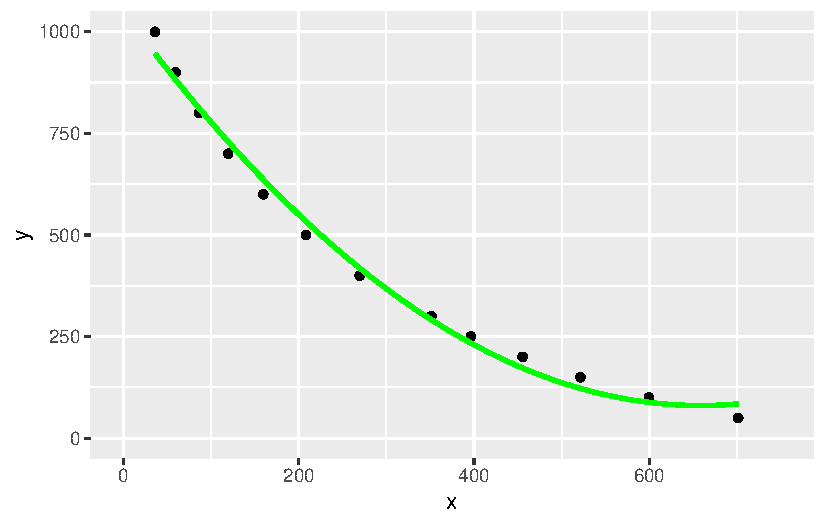
\includegraphics{02-regression-models_files/figure-pdf/unnamed-chunk-6-1.pdf}

Til slutt brukte vi følgende koder for å estimere molekylstørrelsen på
genene i prøven vår.

\begin{Shaded}
\begin{Highlighting}[]
\CommentTok{\# Fit the model}
\NormalTok{cal }\OtherTok{\textless{}{-}} \FunctionTok{lm}\NormalTok{(}\FunctionTok{log}\NormalTok{(mw) }\SpecialCharTok{\textasciitilde{}}\NormalTok{ dist, }\AttributeTok{data =}\NormalTok{ ladder)}

\CommentTok{\# Check model performance, R\^{}2 should be \textasciitilde{} 1.}
\FunctionTok{summary}\NormalTok{(cal)}
\end{Highlighting}
\end{Shaded}

\begin{verbatim}

Call:
lm(formula = log(mw) ~ dist, data = ladder)

Residuals:
      Min        1Q    Median        3Q       Max 
-0.244363 -0.040218 -0.004565  0.082943  0.112630 

Coefficients:
              Estimate Std. Error t value Pr(>|t|)    
(Intercept)  7.0915695  0.0480419  147.61  < 2e-16 ***
dist        -0.0041842  0.0001298  -32.23 3.06e-12 ***
---
Signif. codes:  0 '***' 0.001 '**' 0.01 '*' 0.05 '.' 0.1 ' ' 1

Residual standard error: 0.09807 on 11 degrees of freedom
Multiple R-squared:  0.9895,    Adjusted R-squared:  0.9886 
F-statistic:  1039 on 1 and 11 DF,  p-value: 3.059e-12
\end{verbatim}

\begin{Shaded}
\begin{Highlighting}[]
\CommentTok{\# Estimate molecular weights from migration distances}
\NormalTok{preds }\OtherTok{\textless{}{-}} \FunctionTok{exp}\NormalTok{(}\FunctionTok{predict}\NormalTok{(cal, }\AttributeTok{newdata =}\NormalTok{ unknown)) }
\end{Highlighting}
\end{Shaded}

Brønn 1: 407 bp Brønn 2: 401 bp Brønn 3: 396 bp og 296 bp

\subsubsection{Diskusjon}\label{diskusjon}

Denne analysen viser at ingen av genene våre har helt riktig størelse i
forhold til genene vi testet for - R/R (413bp) og X/X (318bp). Vi er
likevel i nærheten som kan tyde på at allelene for brønn 1 og 2 er R/R
og brønn 3 er R/X. Avviket kan forklares med unøyaktighet under
DNA-testen (sansynlig ettersom validitetskontrollen i prøveresultatet
ikke kom fram) og med dårlig kvalitet på bildet som vi brukte i denne
oppgaven. I rapporten fra forsøket tolket vi prøvene annerledes og
trodde at brønn 1, 2 og 3 alle hadde alleler litt over 300bp og at brønn
3 i tillegg hadde en feil med en ukjent allel som var på 250bp. Dette
viser at det er mye unæyaktighet ved å bruke kun øynene til å tolke
resultatet.

\subsection{Del 3: Tolkning av
regresjonsmodell}\label{del-3-tolkning-av-regresjonsmodell}

\subsubsection{Introduksjon}\label{introduksjon-2}

I denne delen av oppgaven har vi valgt å se nærmere på variablene
FAST\_NUCLEI\_T1 og TRAINING\_AGE i datasettet \texttt{hypertrofi}, som
er en del av \texttt{exscidata} pakken. For utforming av tabeller,
figurer og grafer bruker vi \texttt{tidyverse}, \texttt{broom} og
\texttt{gt}.

\begin{Shaded}
\begin{Highlighting}[]
\CommentTok{\# Laster inn nødvendige biblioteker}
\FunctionTok{library}\NormalTok{(exscidata)}
\FunctionTok{library}\NormalTok{(tidyverse)}
\FunctionTok{library}\NormalTok{(gt)}
\FunctionTok{library}\NormalTok{(broom)}
\end{Highlighting}
\end{Shaded}

I \texttt{?hypertrofi} er FAST\_NUCLEI\_T1 beskrevet som antall
myonuclei per type-II muskelfiber, mens TRAINING\_AGE viser til antall
år med tidligere treningserfaring. Antall myonuclei per type-II
muskelfiber, kan ha noko å si om muskelens egenskap til å utvikle kraft
og personers styrke (McArdle et al., 2014, kap 22). Det er også
diskutert om trening kan føre til endringer i muskelfiber type eller om
de genetiske faktorene er det som er avgjørende for muskelfiber type
fordelingen til den enkelte (McArdle et al., 2014, p. s.535). Vi ønsker
derfor å se nærmer om det er en lineær sammenheng mellom
FAST\_NUCLEI\_T1 og TRAINING\_AGE i datasettet \texttt{hypertrofi}.

\textbf{Spørsmålet}: Er det et lineært forhold mellom myonuclei per
fiber CSA i type 2 og treningsalder?

\subsubsection{Metode}\label{metode-2}

Under i Figure~\ref{fig-plot-training-age-myonuclei} er
\texttt{FAST\_NUCLEI\_T1} satt som den avhengige variabelen på y-aksen,
mens \texttt{TRAINING\_AGE} er valgt som den uavhengige variabelen på
x-aksen. Grafen er ment for å gi oss et raskt overblikk av dataene.

\begin{Shaded}
\begin{Highlighting}[]
\CommentTok{\# Laster inn data}
\FunctionTok{data}\NormalTok{(}\StringTok{"hypertrophy"}\NormalTok{)}

\CommentTok{\# Filtrerer ut NA{-}verdier før du velger variabler}
\NormalTok{ds }\OtherTok{\textless{}{-}}\NormalTok{ hypertrophy }\SpecialCharTok{\%\textgreater{}\%}
  \FunctionTok{filter}\NormalTok{(}\SpecialCharTok{!}\FunctionTok{is.na}\NormalTok{(TRAINING\_AGE) }\SpecialCharTok{\&} \SpecialCharTok{!}\FunctionTok{is.na}\NormalTok{(FAST\_NUCLEI\_T1)) }\SpecialCharTok{\%\textgreater{}\%}
  \FunctionTok{select}\NormalTok{(PARTICIPANT, GROUP, TRAINING\_AGE, FAST\_NUCLEI\_T1)}

\CommentTok{\# Plotter data uten NA{-}verdier}
\NormalTok{ds }\SpecialCharTok{\%\textgreater{}\%} 
  \FunctionTok{ggplot}\NormalTok{(}\FunctionTok{aes}\NormalTok{(TRAINING\_AGE, FAST\_NUCLEI\_T1)) }\SpecialCharTok{+}
  \FunctionTok{geom\_point}\NormalTok{(}\AttributeTok{size =} \DecValTok{2}\NormalTok{, }\AttributeTok{fill =} \StringTok{"red"}\NormalTok{) }\SpecialCharTok{+}
  \FunctionTok{geom\_smooth}\NormalTok{(}\AttributeTok{method =} \StringTok{"lm"}\NormalTok{, }\AttributeTok{se =} \ConstantTok{TRUE}\NormalTok{) }\SpecialCharTok{+}
  \FunctionTok{labs}\NormalTok{(}
    \AttributeTok{title =} \StringTok{"Sammenheng mellom treningserfaring og myonuklei"}\NormalTok{,}
    \AttributeTok{x =} \StringTok{"Treningsår"}\NormalTok{, }
    \AttributeTok{y =} \StringTok{"Myonuklei per fiber CSA i Type II"}\NormalTok{) }\SpecialCharTok{+}
  \FunctionTok{theme\_minimal}\NormalTok{()}
\end{Highlighting}
\end{Shaded}

\begin{figure}[H]

\centering{

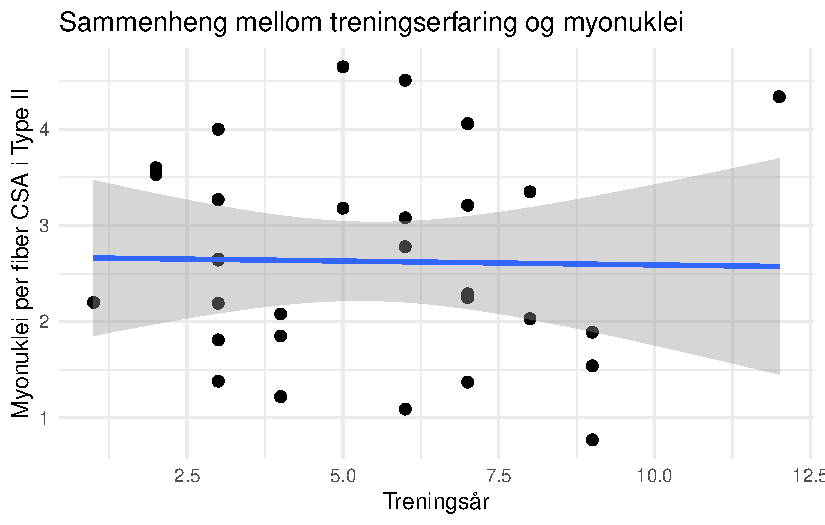
\includegraphics{02-regression-models_files/figure-pdf/fig-plot-training-age-myonuclei-1.pdf}

}

\caption{\label{fig-plot-training-age-myonuclei}Sammenheng mellom
treningalder og myonuclei per fiber CSA i Type-II}

\end{figure}%

ved hjelp av \texttt{geom\_smooth} har vi lagt inn den best tilpassede
linjen til datapunktene, også kalt lineær regresjonslinje
(Spiegelhalter, 2019, pp. s.128--129). Det gråe området omkring
regresjonslinjen, visualiserer konfidensintervallet til linjen. Et bredt
konfidensintervall som fremstilt her, indikerer større usikkerhet i
hvordan variablene relaterer til hverandre (Spiegelhalter, 2019, pp.
s.240--244).

For å presentere regresjonslinjen, har vi laget en lineær statistisk
modell for hjelp til videre tolkning mellom forholdet av dei to
variablene. Oppsummering av de statistiske parametrene som vi har valgt
å fokusere på i diskusjonen vår er listet opp i
Table~\ref{tbl-regresjon} under.

\begin{table}

\caption{\label{tbl-regresjon}Sammenheng mellom treningserfaring og
myonuklei per muskelfiber type-II}

\centering{

\begin{Shaded}
\begin{Highlighting}[]
\CommentTok{\# Lager lineær modell med ds uten NA{-}verdier}
\NormalTok{mod1 }\OtherTok{\textless{}{-}} \FunctionTok{lm}\NormalTok{(FAST\_NUCLEI\_T1 }\SpecialCharTok{\textasciitilde{}}\NormalTok{ TRAINING\_AGE, }\AttributeTok{data =}\NormalTok{ ds)}

\CommentTok{\# Henter ut koeffisienter og deres statistikker}
\NormalTok{model\_summary }\OtherTok{\textless{}{-}} \FunctionTok{tidy}\NormalTok{(mod1)}

\CommentTok{\# Tilpasser p{-}verdier og runder av, og fjerner interceptet}
\NormalTok{model\_summary }\OtherTok{\textless{}{-}}\NormalTok{ model\_summary }\SpecialCharTok{\%\textgreater{}\%}
  \FunctionTok{mutate}\NormalTok{(}
    \AttributeTok{term =} \FunctionTok{ifelse}\NormalTok{(term }\SpecialCharTok{==} \StringTok{"(Intercept)"}\NormalTok{, }\StringTok{"Intercept (Konstantledd)"}\NormalTok{, }\StringTok{"Treningserfaring (år)"}\NormalTok{),}
    \AttributeTok{p.value =} \FunctionTok{ifelse}\NormalTok{(p.value }\SpecialCharTok{\textless{}} \FloatTok{0.001}\NormalTok{, }\StringTok{"\textless{} 0.001"}\NormalTok{, }\FunctionTok{round}\NormalTok{(p.value, }\DecValTok{3}\NormalTok{)),}
    \AttributeTok{estimate =} \FunctionTok{round}\NormalTok{(estimate, }\DecValTok{3}\NormalTok{),}
    \AttributeTok{std.error =} \FunctionTok{round}\NormalTok{(std.error, }\DecValTok{3}\NormalTok{),}
    \AttributeTok{statistic =} \FunctionTok{round}\NormalTok{(statistic, }\DecValTok{3}\NormalTok{)}
\NormalTok{  ) }\SpecialCharTok{\%\textgreater{}\%}
  \CommentTok{\# Filtrer ut interceptet}
  \FunctionTok{filter}\NormalTok{(term }\SpecialCharTok{!=} \StringTok{"Intercept (Konstantledd)"}\NormalTok{)}
  \CommentTok{\# Velger å filtrere ut intercept da det ikkje er aktuelt når vi kun skal se om}
  \CommentTok{\# det er en lineær sammenheng mellom dei to variablene}

\CommentTok{\# Lager regresjonstabell med forklarende radnavn}
\NormalTok{regression\_table }\OtherTok{\textless{}{-}}\NormalTok{ model\_summary }\SpecialCharTok{\%\textgreater{}\%}
  \FunctionTok{select}\NormalTok{(term, estimate, std.error, statistic, p.value) }\SpecialCharTok{\%\textgreater{}\%}
  \FunctionTok{gt}\NormalTok{() }\SpecialCharTok{\%\textgreater{}\%}
  \FunctionTok{fmt\_auto}\NormalTok{() }\SpecialCharTok{\%\textgreater{}\%}
  \FunctionTok{cols\_label}\NormalTok{(}
    \AttributeTok{term =} \StringTok{"Term"}\NormalTok{,}
    \AttributeTok{estimate =} \StringTok{"Estimert koeffisient"}\NormalTok{,}
    \AttributeTok{std.error =} \StringTok{"Standardfeil"}\NormalTok{,}
    \AttributeTok{statistic =} \FunctionTok{md}\NormalTok{(}\StringTok{"*t*{-}verdi"}\NormalTok{),}
    \AttributeTok{p.value =} \FunctionTok{md}\NormalTok{(}\StringTok{"*p*{-}verdi"}\NormalTok{)}
\NormalTok{  ) }\SpecialCharTok{\%\textgreater{}\%}
  \FunctionTok{tab\_source\_note}\NormalTok{(}
    \AttributeTok{source\_note =} \StringTok{"**Notat**: *p*{-}verdier mindre enn 0.05 anses som statistisk signifikante."}
\NormalTok{  )}

\CommentTok{\# Vis resultatene}
\FunctionTok{print}\NormalTok{(regression\_table)}
\end{Highlighting}
\end{Shaded}

\phantomsection\label{tubbivpoow}
Term

Estimert koeffisient

Standardfeil

t-verdi

p-verdi

Treningserfaring (år)

−0.008

0.077

−0.104

0.918

\textbf{Notat}: \emph{p}-verdier mindre enn 0.05 anses som statistisk
signifikante.

}

\end{table}%

\subsubsection{Diskusjon}\label{diskusjon-1}

I tabellen kan vi lese av verdiene for estimert koeffisient
(regresjonskoeffisient), standardfeil, t-verdi og p-verdi. Den estimerte
koeffisenten til ``Treningserfaring (år)'' forteller oss hvor mye
\texttt{FAST\_NUCLEI\_T1} endres per enhet økning i
\texttt{TRAINING\_AGE}. I vårt tilfelle ser man en antall nukleikjerner
per fiber reduseres med 0.008 per år med treningserfaring.

Standardfeilen måler hvor mye koeffisientene er forventet å variere fra
utvalg til utvalg. Standardfeilen som vi har fått er liten i tallverdi,
og man kan da fort konkludere at estimeringen er presis grunnet lav
standardfeil. Samtidig er det viktig å se standardfeilen i lys av den
estimerte koefisienten. I forhold til koeffisienten selv, er
standardfeilen stor, og betyr at man burde være usikker på nøyaktigheten
til estimatet (Spiegelhalter, 2019, pp. s.230--232)

\emph{t-verdien} sier hvor mange standardavvik den estimerte
koeffisienten er fra 0, der jo høyere t-verdien (enten negativ eller
positiv), dess mer signifikant er koeffisienten (Spiegelhalter, 2019,
pp. s.275--276). Hos oss er t-verdien -0.104, noe som indikerer at det
ikke er noe signifikant lineær sammenheng mellom
\texttt{FAST\_NUCLEI\_T1} og \texttt{TRAINING\_AGE}.

Nært knyttet til t-verdien, har man \emph{p-verdien} som hjelper oss å
si om t-verdien er statistisk signifikant. P-verdi er sannsynligheten
for å observere en så ekstrem teststatistikk som den t-verdien vi har
fått, gitt antagelsen at det ikke er en sammenheng mellom variablene
våre (Spiegelhalter, 2019, pp. s.264--265). Basert på at p-verdien i vår
modell er 0.918, er det 91,8 \% sannsynlighet at man vil observere en
t-verdi på -0.008. Vi har derfor ikkje tilstrekkelig bevis for å kunne
si at den uavhengige variabelen \texttt{TRAINING\_AGE} har en effekt på
den avhengige variabelen \texttt{FAST\_NUCLEI\_T1}, og at det er en
statistik lineær sammenheng mellom variablene (Spiegelhalter, 2019, pp.
s.265--268).

Selv om p-verdi er et nyttig verktøy for å hjelpe oss å trekke
slutninger om koeffisientenes statistiske signifikans, sier den oss ikke
noe om størrelsen på en effekt eller hva praktisk betydning den kan ha.
Størrelsen på datasettet har også en betydning på p-verdien, der små
datasett, som det vi har, kan gi høye p-verdier selv om det er en
betydelig effekt (Spiegelhalter, 2019, p. s.285)

\phantomsection\label{refs}
\begin{CSLReferences}{1}{0}
\bibitem[\citeproctext]{ref-machado2012}
Machado, F. A., Nakamura, F. Y., \& Moraes, S. M. F. D. (2012).
Influence of regression model and incremental test protocol on the
relationship between lactate threshold using the maximal-deviation
method and performance in female runners. \emph{Journal of Sports
Sciences}, \emph{30}(12), 1267--1274.

\bibitem[\citeproctext]{ref-mcardle2014}
McArdle, W. D., Katch, F. I., \& Katch, V. L. (2014). \emph{Exercise
physiology: Nutrition, energy, and human performance} (8th ed.). Wolters
Kluwer Health.

\bibitem[\citeproctext]{ref-spieg2019}
Spiegelhalter, D. J. (2019). \emph{The art of statistics : Learning from
data} (1th ed.). Pelican.

\end{CSLReferences}




\end{document}
